\documentclass{article}
\usepackage{natbib}
\usepackage[francais]{babel}
\usepackage[utf8]{inputenc}
\usepackage[T1]{fontenc}
\usepackage{hyperref}
\usepackage{graphicx}
\usepackage{minted}
\usepackage{uqac}
\usepackage{sectioncompilation}

% ================================ Meta data (pour titre et autre)
\discipline{8INF844}
\supervisor{Abdenour Bouzouane}
\project{TP1}
\title{Simulation multi-agents avec NetLogo}
\author{Sébastien Blin\\Victor Drouin Viallard}

% ================================ Document
\begin{document}

\maketitle

\section{Synthèse de l'article}
\subsection{Introduction}
L'article \emph{Flocks, Herds, and Schools: A Distributed Behavioral Model} (\emph{Craig W. Reynolds}) décrit comment simuler des flocks en considérant chaque individu à part, sans avoir à programmer un mouvement pour chaque individu mais plutôt en le calculant à partir de l'environnement qu'il perçoit. Le flock sera ainsi le résultat du mouvement de chaque individu. À première vue, la simulation d'un flock peut paraître difficile car il y a beaucoup d'individus à simuler et l'environnement est très dur à maintenir (éviter les collisions entre toutes les particules à chaque frame par exemple), mais ce papier propose une méthode pour réussir à simuler ce mouvement sans avoir à réaliser la gestion des collisions. Ainsi le flock sera le résultat du comportement d'un seul individu appliqué à tous les oiseaux.

On considère ici le flock comme un ensemble de particules améliorées (\emph{boid}) : chaque particule représente un individu (ici un oiseau) et possède des variables (couleur, localisation, velocité, etc) auxquelles on donne une forme - donc une notion d'orientation - ainsi qu'une vitesse maximale.

\subsection{Fonctionnement de l'algorithme}
Les observations montre que certains animaux se regroupent en flock afin de se protéger des prédateurs, chercher de la nourriture, etc. Pour participer à un flock, un oiseau doit pouvoir se coordoner avec les oiseaux qui l'entourent. Vu qu'un flock est possiblement infini en taille (certains bancs de poissons ont des millions d'individus), on suppose que l'animal ne considère que lui-même, quelques uns de ses voisins et l'ensemble du flock. On peut alors considérer trois forces~:

\begin{itemize}
  \item \emph{Collision Avoidance}, pour éviter de rentrer en collision avec les autres oiseaux.
  \item \emph{Velocity Matching}, pour avoir la direction et la vitesse des oiseaux voisins.
  \item \emph{Flock Centering}, pour rester proche des oiseaux voisins et aller vers le centre du flock
\end{itemize}

On observe deux forces opposées~: l'une qui pousse l'oiseau à rester dans le flock, l'autre qui le pousse à éviter les autres oiseaux~; il faut y prêter attention car cela peut amener l'oiseau à ne pas savoir où se déplacer.

Les trois forces agissent indépendament et propose une solution différente au choix de la direction à prendre. On peut alors décider d'atténuer plus ou moins telle ou telle force et les combiner pour obtenir le mouvement résultant des 3 forces, etc. Si faire la moyenne de ces trois forces est la solution la plus simple, il semble plus intéressant de les prioritiser puis de les accumuler dans l'ordre jusqu'à atteindre une magnitude totale maximale pour éviter les problèmes d'opposition évoqués précédemment. Par exemple, si on regarde en priorité la force de \emph{Collision Avoidance} et qu'elle est de magnitude plus forte que celle maximale alors on suivra directement cette force pour éviter en priorité la collision et les autres forces seront temporairement inutilisées.

\subsection{Améliorations possibles}
On peut enfin ajouter des fonctionnalités comme l'ajout d'obstacles et leur évitement, l'initialisation de la position des oiseaux, ou encore leur donner un but de migration (éléments à récupérer). La plus intéressante des fonctionnalités est l'évitement d'objets. Pour la réaliser, deux solutions sont envisageables. La première, \emph{force field concept}, consiste à avoir une force de répulsion autour de l'objet à éviter mais si l'oiseau arrive pile en face d'une ligne du champ, il ne sera pas repoussé mais ralenti jusqu'à se bloquer. De plus si l'oiseau vole à coté d'un mur il n'a pas besoin de tourner même si celui-ci est dans le champ de vision; ce qui nous amène à la seconde, \emph{steer-to-avoid}, où l'oiseau ne considère que les obstables face à lui. S'il en trouve un, il calcule alors un vecteur afin d'éviter l'objet.

\subsection{Conclusion}
On peut trouver plusieurs applications concrètes à la simulation d'un flocking comme par exemple dans la simulation de traffics routiers ou encore pour l'observation et la prévision du comportement d'animaux.
Enfin, il est possible d'améliorer l'algorithme en le parrallélisant ou en étant sûr que $N$ soit assez petit (en considérant seulement une partie du flock par exemple, sans quoi la complexité rebute).

\section{Modification du code source}

Le Flock se base donc sur 3 forces, séparées en 3 fonctions dans le code prenant chacune en paramètre la liste des individus voisins~:
\begin{itemize}
  \item \emph{separate}, pour empêcher que les individus rentrent en collision. Ici, un vecteur force est calculé entre un individu et les voisins qu'il détecte. Ce vecteur est alors pondéré par l'inverse de la distance entre chaque couble d'individus. Ainsi, plus les individus sont proches, plus la force de séparation sera forte.
  \begin{figure}[h]
  	\begin{center}
  		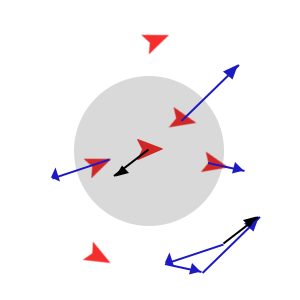
\includegraphics[scale=0.3]{img/separate}
  		\caption{Force de séparation}
  		\label{fig:separate}
  	\end{center}
  \end{figure}
  \item \emph{align}, qui sert à aligner les individus dans la même direction pour générer un mouvement migratoire. Ici on prend les vecteurs d'alignement de chaque individus dans le voisinage, et on considère leur moyenne.
  \begin{figure}[h]
  	\begin{center}
  		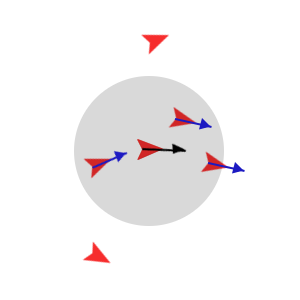
\includegraphics[scale=0.3]{img/align}
  		\caption{Force d'alignement}
  		\label{fig:align}
  	\end{center}
  \end{figure}
  \item \emph{cohere} qui resulte en une force poussant l'individu vers le centre de gravité de ses voisins.
  \begin{figure}[h]
  	\begin{center}
  		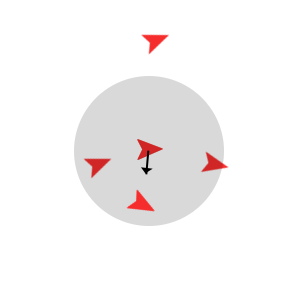
\includegraphics[scale=0.3]{img/cohere}
  		\caption{Force de cohésion}
  		\label{fig:cohere}
  	\end{center}
  \end{figure}
\end{itemize}

\section{Ramassage d'objets}

De plus nous pouvons désormais générer des objets aléatoires sur le terrain. Les oiseaux peuvent alors prendre ces objets et le lacher lorsqu'un objet du même type se situe à côté de ce point. Un oiseau ne peut pas prendre plusieurs objets. L'idée est donc de former progressivement des tas avec les objets générés.
2 scénarios ont été réalisés (cf ci dessous). Soit l'agent récupère un objet et le garde jusqu'à la fin, soit il peut le lacher afin de former des tas. Dans le deuxième cas s'il ne parvient pas à poser son objet à une position adéquate après un certain temps l'individu l'abandonnera pour en trouver un autre.

\section{Pondération des forces}

Nous avons tenté plusieurs scénarios et nous obtenons un résultat qui fonctionne avec la configuration suivante~:
\begin{itemize}
  \item population 200
  \item align-factor 5,5
  \item cohere-factor 0,4
  \item separate-factor 4,0 (avec minimum-separation d'une valeur de 2,5 et une vision de 8 patches)
\end{itemize}
On remarque que la force de cohésion est plus forte que les deux autres forces d'où sa multiplication par un facteur faible.

\section{Mesure de performance}

Afin de mesurer la performance du flock, nous avons décidé de mesurer le nombre de voisins détectés par un individu arbitraire ($turtle 0$). Ainsi, si le flock fonctionne, le nombre de voisin devrait augmenter avec le temps.

\begin{figure}[h]
	\begin{center}
		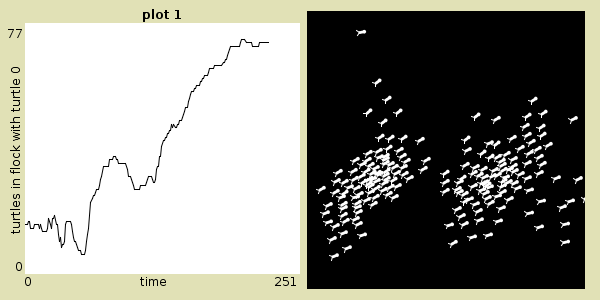
\includegraphics[scale=0.5]{img/performance}
		\caption{Performance avec les pondérations données précédement}
		\label{fig:performance}
	\end{center}
\end{figure}

\section{Pondération d'un non-flock}
Si la force de cohésion est nulle les agents ne se comporteront plus en flock, peu importe les valeurs des deux autres forces. Le ramassage d'objets pour en faire des tas est beaucoup plus lent (mais continue de fonctionner car les agents reste en général dans une direction commune).

\section{Création de tas}

Pour cette question nous avons décidé de rajouter deux forces pour remplacer la force d'alignement et celle de cohésion. Ces deux nouvelles forces fonctionnent exactement de la même manière mais sont alors uniquement considéré les voisins de même couleur pour les calculs.

La force de séparation n'a pas été modifiée car quelque soit la couleur les collisions doivent être évitées. Enfin pour cette question nous conseillons désactivé les dépos d'objets (mettre \emph{drop} à off) : ainsi lorsqu'un oiseau prend un objet il le garde jusqu'à la fin et il est plus facile de voir se former des flocks de même couleur.

Pour utiliser convenablement la notion de couleur il est conseillé de mettre à 0 les valeurs de align-factor et cohere-factor pour joueur sur les valeurs de color-align-factor et color-cohere-factor.

On commence à voir des groupes se former avec les paramètres ci-dessus au bout de 2000 ticks environ.
\section{Interface}
\begin{figure}[h]
	\begin{center}
		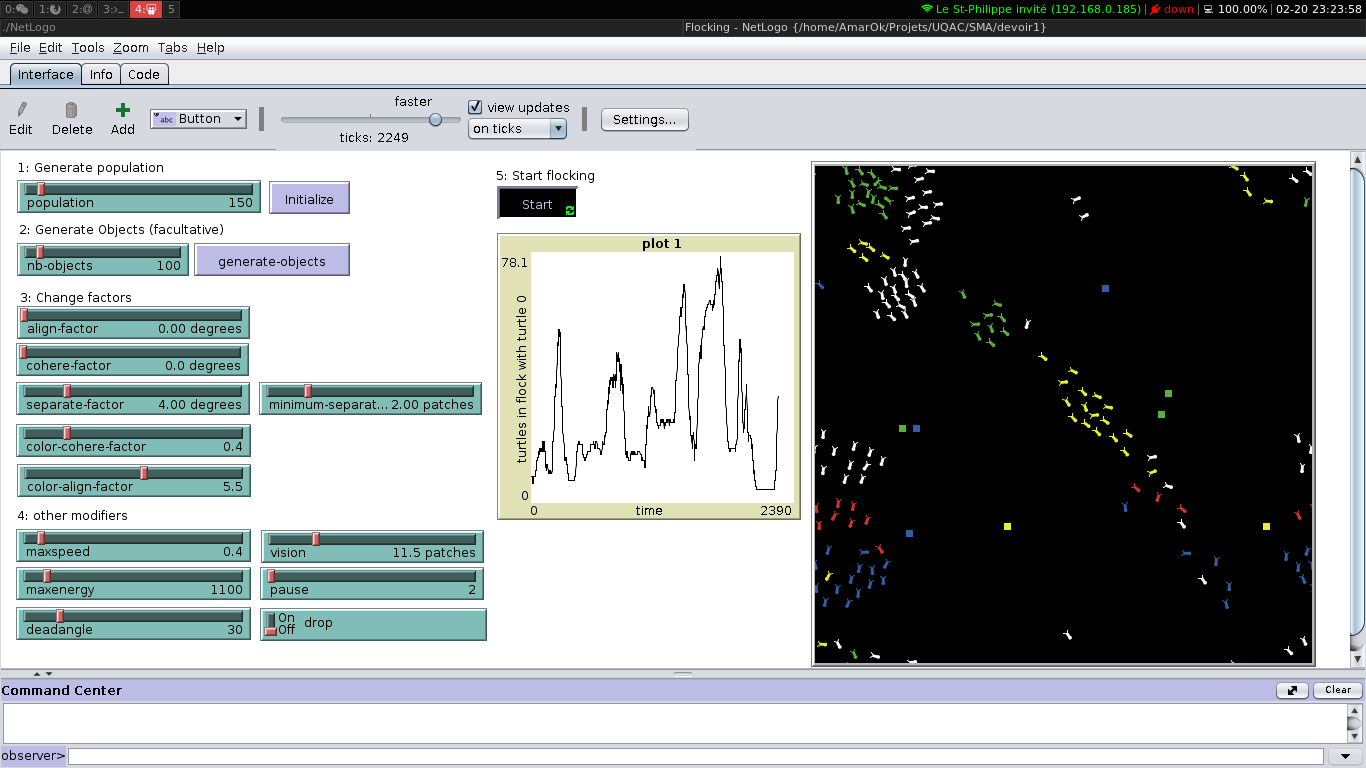
\includegraphics[scale=0.3]{img/groups}
		\caption{Des groupes de flocks}
		\label{fig:groups}
	\end{center}
\end{figure}

\section{Comparaison des 2 flocks}
Au final, outre le fait que l'exemple de flocking de NetLogo soit plus basique (pas de gestion de récupération d'objet, d'énergie, de formations de tas, etc.), la séparation du modèle précédent ne se base que sur le voisin le plus proche ce qui fait qu'un agent rebondi dans le cas où l'agent possède un voisin de chaque côté alors qu'avec notre modèle, l'agent restera environ entre les deux agents. Le mouvement sera donc plus naturel.
De plus le fait de limiter le mouvement avec une limite de degrés pour les forces de cohésion et d'alignement n'est pas forcément pertinent d'un point de vue naturel, un oiseau pouvant généralement changer de direction relativement rapidement. Cependant, il possède pour avantage d'être simple et peu gourmand en calculs pour NetLogo.

\section{Ajout de fonctionnalités}

Deux fonctionnalités ont été ajoutées.

\paragraph{Energie}
La première est la consommation d'énergie. Chaque agent possède un niveau d'énergie entre 1 et $maxenergy$. Cette charge baisse de 1 par tick. Une fois que l'agent n'a plus d'énergie, il s'arrête, lâche l'objet s'il en possède un et se met en pause. Il possède ensuite $1/pause$ probabilité de repartir à chaque tick. En repartant il choisit une nouvelle direction.

\paragraph{Champ de vision}
La seconde fonctionnalité est le champ de vision. L'agent possède un angle mort à l'arrière qui est paramétrable avec une valeur entre 0° et 180°. Par exemple, lorsque cette valeur est paramétrée à 30°, l'agent possède donc un angle mort de 60° à l'arrière. Si un autre agent se trouve dans cet angle, il est ignoré et ne sera pas comptabilisé parmi ses voisins.

\section{Interface}
\begin{figure}[h]
	\begin{center}
		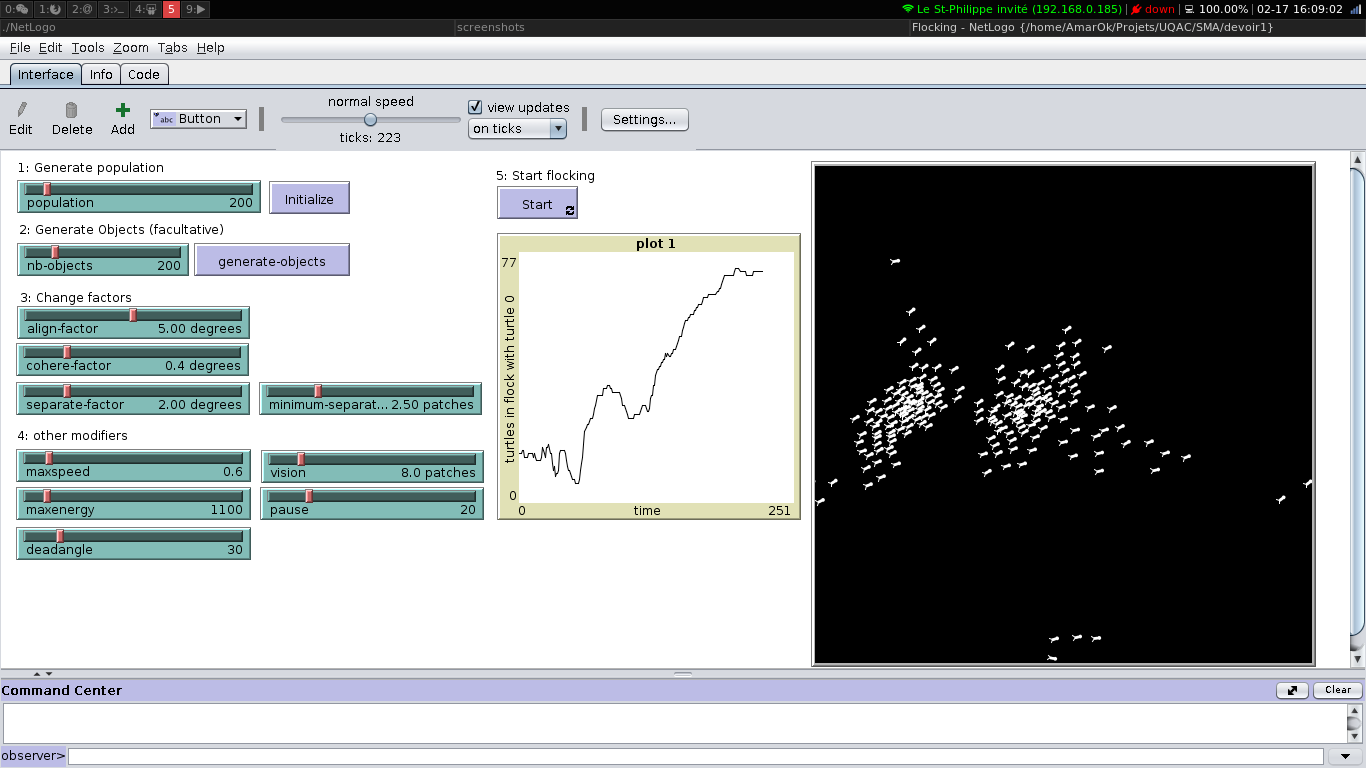
\includegraphics[scale=0.3]{img/interface}
		\caption{Interface finale}
		\label{fig:interface}
	\end{center}
\end{figure}

\end{document}
